\documentclass{ctexart}
% \usepackage[UTF-8]{ctex}
\usepackage{amsmath}
\usepackage{booktabs}
\usepackage{multirow}
\usepackage{tabularx}

\usepackage{booktabs,multirow,longtable}

\usepackage{listings}
\usepackage{listings}
\usepackage{color}

%导言区插入下面三行
\usepackage{graphicx} %插入图片的宏包
\usepackage{float} %设置图片浮动位置的宏包
\usepackage{subfigure} %插入多图时用子图显示的宏包


\definecolor{dkgreen}{rgb}{0,0.6,0}
\definecolor{gray}{rgb}{0.5,0.5,0.5}
\definecolor{mauve}{rgb}{0.58,0,0.82}

\lstset{frame=tb,
  language=Python,
  aboveskip=3mm,
  belowskip=3mm,
  showstringspaces=false,
  columns=flexible,
  basicstyle={\small\ttfamily},
  numbers=left,
  numberstyle=\tiny\color{gray},
  keywordstyle=\color{blue},
  commentstyle=\color{dkgreen},
  stringstyle=\color{mauve},
  breaklines=true,
  breakatwhitespace=true,
  tabsize=3
}


\title{作业4:有限元方法求解一维微分方程}
\author{谢文进}
\date{\today}
\begin{document}
\maketitle
\section{作业4:有限元方法求解一维微分方程}
\subsection{理论推导}
对于微分方程
$$
    \left\{\begin{matrix}
        -u''=f, \quad  0<x<1 \\ 
        u(0)=0,u'(1)=0.
    \end{matrix}\right.
$$
现在取$f=1$,求解如下方程:

$$
    \left\{\begin{matrix}
        -u''=1, \quad  0<x<1 \\ 
        u(0)=0,u'(1)=0,
    \end{matrix}\right.
$$
上述方程精确解为$u(x)=-\frac{1}{2}x^2+x$.
现在用有限元方法进行数值求解,重要的是计算出总体刚度矩阵$A$以及
载荷向量$b$。
$$
A=
\sum_{i=1}^{N} \begin{pmatrix}
  &  &  &  &  & \\
  &  &  &  &  & \\
  & \cdots & \frac{1}{h_i}  & -\frac{1}{h_i} & \cdots & \\
  & \cdots &  -\frac{1}{h_i}& \frac{1}{h_i} & \cdots & \\
  &  &    &   &  & \\
  &  &  &  &  &
\end{pmatrix}_{(N+1)\times (N+1)}
$$

$$
b=\sum_{i=1}^{N}\frac{h_i}{2}\int_{-1}^{1} \begin{pmatrix}
  0\\
  0\\
  \vdots\\
  f(F(\xi ))N_1(\xi )\\
  f(F(\xi ))N_2(\xi )\\
  0\\
  \vdots \\
 0
 \end{pmatrix}_{(N+1)\times 1} d\xi 
$$
代入$f(x)=1$,可以得到
$$
\int_{-1}^{1} f(F(\xi))N_1(\xi)d\xi=\int_{-1}^{1}\frac{1}{2}(1-\xi)d\xi = 1,
$$

$$
\int_{-1}^{1} f(F(\xi))N_2(\xi)d\xi=\int_{-1}^{1}\frac{1}{2}(1+\xi)d\xi = 1.
$$
因此
$$
b=\sum_{i=1}^{N}\frac{h_i}{2} \begin{pmatrix}
  0\\
  0\\
  \vdots\\
 1\\
  1\\
  0\\
  \vdots \\
 0
 \end{pmatrix}_{(N+1)\times 1} .
$$
现在处理边界条件$u(0)=0,u'(1)=0$,由于$u'(1)=0$在证明过程中自然满足,只需处理边界
条件$u(0)=0$.记$Au=b$,即
$$
\begin{pmatrix}
  a_{00}& a_{01} & \cdots  & a_{0N} \\
  a_{10} &  a_{11} &  \cdots & a_{1N} \\
 \cdots  & \cdots  & \cdots  & \cdots  \\
 a_{N0} & a_{N1} & \cdots  & a_{NN}
\end{pmatrix}
\begin{pmatrix}
 u_0\\
 u_1\\
 \vdots\\
u_N
\end{pmatrix}=
\begin{pmatrix}
 b_0\\
 b_1\\
 \vdots\\
b_N
\end{pmatrix}.
$$
由此可得
$$
\begin{matrix}
  a_{01}u_1+\cdots +a_{0N}u_N=b_0-a_{00}u_0\\
  a_{11}u_1+\cdots +a_{1N}u_N=b_1-a_{10}u_0\\
  \cdots \\
 a_{N1}u_1+\cdots +a_{NN}u_N=b_N-a_{N0}u_0
 \end{matrix}
$$
加入一个方程$1\times u_0 + 0 \times u_1 + \cdots +0 \times u_N = u_0$,写成矩阵形式得到:
$$
\begin{pmatrix}
  1 & 0 & \cdots & 0 \\
  0 & a_{11} & \cdots  & a_{1N}\\
  \vdots & \vdots &  & \vdots\\
  0 & a_{N1} & \cdots & a_{NN}
 \end{pmatrix}
 \begin{pmatrix}
  u_0\\
  u_1\\
  \vdots\\
 u_N
 \end{pmatrix}=
 \begin{pmatrix}
  u_0\\
  b_1\\
  \vdots\\
 b_N
 \end{pmatrix}-
 \begin{pmatrix}
 0 \\
 a_{10} \\
 \vdots \\
 a_{N0}
 \end{pmatrix}u_0,
$$
代入$u_0=0$得到最终的方程组
$$
\begin{pmatrix}
  1 & 0 & \cdots & 0 \\
  0 & a_{11} & \cdots  & a_{1N}\\
  \vdots & \vdots &  & \vdots\\
  0 & a_{N1} & \cdots & a_{NN}
 \end{pmatrix}
 \begin{pmatrix}
  u_0\\
  u_1\\
  \vdots\\
 u_N
 \end{pmatrix}=
 \begin{pmatrix}
  0\\
  b_1\\
  \vdots\\
 b_N
 \end{pmatrix},
$$
求解上述方程组即可得到数值解$u$。
\subsection{编程实现}
根据上述推导,用python编写程序,代码如下:

\begin{lstlisting}
  import numpy as np
  import math
  from scipy import linalg # 求解方程组需要引用的包
  import matplotlib.pyplot as plt # 画图
  
  # 求解微分方程 -u'' = 1, u(0) = 0, u'(1) = 0
  # 精确解为 u(x) = -0.5 * x^2 + x
  x0 = 0.0 
  xN = 1.0
  N = 10  # 节点x0, x1, ..., xN
  h = (xN - x0) / N 
  
  # 精确解 u(x) = -0.5 * x^2 + x
  def exactf(x):
      return (-1) * 0.5 * x * x + x
  
  # f(F(\xi))N1(\xi)在[-1,1]上的积分值
  def integrate_f1():
      return 1
  
  # f(F(\xi))N2(\xi)在[-1,1]上的积分值
  def integrate_f2():
      return 1
  
  
  # 生成矩阵A和右端项RHS
  def generate(N, f1, f2):
      A = np.zeros([N+1, N+1])
      RHS = np.zeros([N+1,1])
      for i in range(1, N+1):
          A[i,i] += 1/h
          A[i-1, i-1] += 1/h
          A[i-1,i] += -1/h
          A[i,i-1] += -1/h
          RHS[i] += (h/2) * f1 
          RHS[i-1] += (h/2) * f2 
      return A,RHS
  
  
  # 处理边界条件 u(0) = 0
  def modified_matrix(A, RHS, u0, uN):
      # 1. 先更新右端项
      # 处理边界条件u0
      for i in range(1,N):
          RHS[i] = RHS[i] - A[i,0] * u0
      RHS[0] = u0
  
      # # 处理边界条件uN,当给出u(xN)的值时,取消注释
      # for i in range(1,N):
      #     RHS[i] = RHS[i] - A[i,N] * uN
      # RHS[N] = uN
      
      # 2. 更改矩阵A
      for i in range(N+1):
          A[0,i] = 0
          A[i,0] = 0
          # A[N,i] = 0 # 当给出u(xN)的值时,取消注释
          # A[i,N] = 0 # 当给出u(xN)的值时,取消注释
      A[0,0] = 1
      # A[N,N] = 1 # 当给出u(xN)的值时,取消注释
      return A,RHS
  
  A,RHS = generate(N,integrate_f1(),integrate_f2())
  A,RHS = modified_matrix(A, RHS, 0, 0)
  
  # 数值解 求解方程组 Ax=RHS
  x = linalg.solve(A, RHS)
  # print(x)
  
  # 精确解
  u = np.zeros([N+1,1])
  for i in range(N+1):
      u[i] = exactf(i * h)
  # print(u)
  
  # 输出误差
  err = max(abs(u - x))
  print(N,err)
  
  # 画图比较精确解和数值解
  t = np.arange(x0, xN + h, h)
  plt.title('Result')
  plt.plot(t, x, color='green', label='numerical solution')
  plt.plot(t, u, color='blue', label='exact solution')
  plt.legend() # show the legend
  
  plt.xlabel('t')
  plt.ylabel('u')
  plt.show()
\end{lstlisting}

\subsection{结果分析}
当取$N=10$,即$h=\frac{1}{N}=0.1$时,精确解$u$与数值解$u_1$图像如图 \ref{Fig.main2} 所示,可以看到两条线几乎重合,计算误差
$||u-u_1||_{\max}=2.22044605e-16$
\begin{figure}[H] %H为当前位置,!htb为忽略美学标准,htbp为浮动图形
  \centering %图片居中
  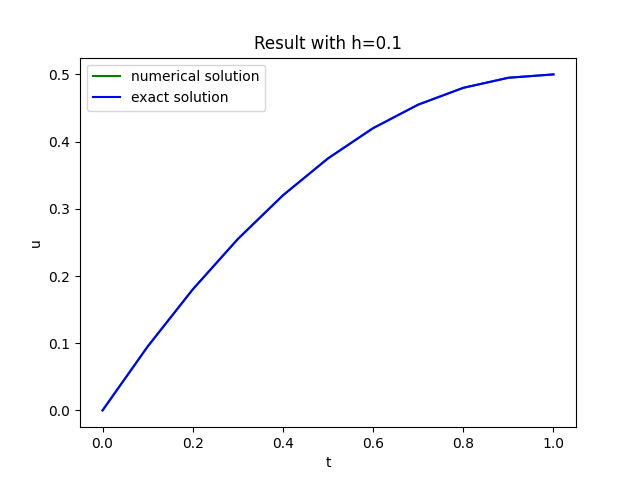
\includegraphics[width=0.7\textwidth]{Figure_1.png} %插入图片,[]中设置图片大小,{}中是图片文件名
  \caption{$h=0.1$结果图} %最终文档中希望显示的图片标题
  \label{Fig.main2} %用于文内引用的标签
\end{figure}
取不同的$h$得到的误差如表\ref{table1}所示。
由上述数值结果可以验证此方法及程序的正确性。

% Please add the following required packages to your document preamble:
% \usepackage{booktabs}
\begin{table}[]
  \centering
  \caption{不同$h$误差表}
  \begin{tabular}{@{}cc@{}}
  \toprule
  h     & error          \\ \midrule
  1/4   & 2.77555756e-16 \\
  1/8   & 5.55111512e-17 \\
  1/16  & 1.11022302e-16 \\
  1/32  & 8.38218384e-15 \\ 
  1/100 & 8.32667268e-15 \\
  1/200 & 6.29496455e-14 \\ \bottomrule
  \end{tabular}
  \label{table1}
  \end{table}


\end{document}